\documentclass[a4paper]{article}
\usepackage[french]{babel}
\usepackage[utf8]{inputenc}
\usepackage[T1]{fontenc}
\usepackage{booktabs}   % For better-looking horizontal lines
\usepackage{array}      % For adjusting row spacing
\usepackage{csquotes}   % pour éviter un warning
\usepackage{graphicx}   % pour les images
\usepackage{hyperref}   % pour les références
\usepackage{float}      % pour les figures
\usepackage{amsmath}    % pour les formules mathématiques
% \usepackage{multicol}   % pour les 2 colonnes
\usepackage{subcaption} % pour les sous-figures
% \usepackage{caption}    % pour les légendes
% \usepackage{fullpage}   % mets les marges en petits 
% \usepackage{placeins}   % For     \FloatBarrier command
\usepackage{appendix}  % For appendices

\usepackage[style=ieee,backend=biber]{biblatex}
\addbibresource{ref.bib}

\hypersetup{
    colorlinks=true,
    linkcolor=blue,   % Couleur des liens internes (table des matières, références)
    citecolor=green,  % Couleur des liens vers les références bibliographiques
    filecolor=magenta,% Couleur des liens vers les fichiers
    urlcolor=blue     % Couleur des liens vers les URL
}

\title{Rapport Projet 3A \\ Analyse de traces de sang}
% \subtitle{Analyse de trace de sang}
\author{Cléa Han, Yanis Labeyrie et Adrien Zabban}
% \institute{Ecole Centrale Méditerranée, 13013 Marseille, France}
\date{Mars 2024}

\begin{document}

\maketitle
% \bigskip
% \tableofcontents
% \newpage

\section{Introduction}

Notre projet 3A s'intéresse à l'analyse de traces de sang dans le cadre du travail de l'expert criminalistique Philippe Esperança. En effet, l'objectif est de réaliser une intelligence artificielle pour assister et faciliter le travail d'analyse de scènes de crimes présentant du sang. 

Les travaux de Philippe Esperança sur l'analyse des traces de sangs~\cite{PhilippeEsperança}, a abouti à la classification de ces traces en 19 classes distinctes qui sont listées dans la Table~\ref{tab:classes}. Notre but est alors de faire un modèle de machine learning capable de prédire la classe pour une image de trace de sang.

\begin{table}[ht]
    \centering
    \begin{tabular}{|ll|}
        \hline
        \textbf{Classe des types de trace de sang} &  \\
        \hline
        1- Modèles Traces passives & 2- Modèles Goutte à Goutte \\
        3- Modèle Transfert par contact & 4- Modèle Transfert glissé \\
        5- Modèle Altération par contact & 6- Modèle Altération glissée \\
        7- Modèle d'Accumulation & 8- Modèle Coulée \\
        9- Modèle Chute de volume & 10- Modèle sang Propulsé \\
        11- Modèle d'éjection & 12- Modèle Volume Impacté \\
        13- Modèle Imprégnation & 14- Modèle Zone d'interruption \\
        15- Modèle d'impact & 16- Modèle Foyer de modèle d'impact \\
        17- Modèle Trace gravitationnelle & 18- Modèle Sang expiré \\
        19- Modèle Trace d'insecte & \\
        \hline
    \end{tabular}
    \caption{Liste des 19 modèles de trace de sang}
    \label{tab:classes}
\end{table}

\section{Données}

Philippe Esperança nous a fourni deux bases de données. La première contient des images de traces de sang reproduites en laboratoire. La deuxième correspond à des images issues de scène de crime.
Cependant, il y avait la présence d'une classe trop minoritaire parmi ces 19 classes, qui est la classe de trace d'insectes possédant uniquement quatre images. Cette classe a donc été retirée afin de garder une certaine distribution relativement équilibrée. Nous avons donc travaillé avec 18 classes.

\subsection{Données de laboratoire}

Dans un premier temps, nous avons pu manipuler des données de laboratoire, c'est-à-dire des images de traces de sang reproduites en laboratoire sur des fonds réguliers, hors des scènes de crimes. Ces fonds sont de quatre types différents : bois, linoleum (lino), carrelage et papier. Ces données sont composées de $10978$ images.
La Figure~\ref{fig: labs images} présente des images de taches de sang reproduites en laboratoire. La Table~\ref{tab: images of all classes} en annexe montre un exemple de trace de sang pour chacune des 18 classes.

\begin{figure}[ht]
    \centering
    \begin{subfigure}{0.35\linewidth}
        \centering
        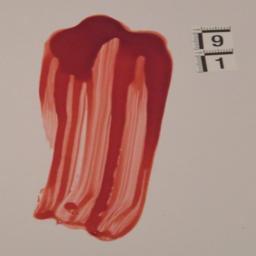
\includegraphics[width=\linewidth]{../asset/data_labo/4_papier_1586.jpg}
        \caption{Modèle Transfert glissé sur un fond de papier}
    \end{subfigure}
    \begin{subfigure}{0.35\linewidth}
        \centering
        \includegraphics[width=\linewidth]{../asset/data_labo/8_coulée_4526.jpg}
        \caption{Modèle de Coulée sur fond de lino}
    \end{subfigure}
    \caption{Deux images de laboratoire}
    \label{fig: labs images}
\end{figure}

Nous avons réparti ces données de laboratoire en 80\% dans nos données d'entraînement, 10\% dans nos données de validation et 10\% dans nos données de test. La Figure~\ref{fig:distribution labo} nous montre la distribution des données de laboratoire sur chacune des classes et chacun des datasets.

\begin{figure}[ht]
    \centering
    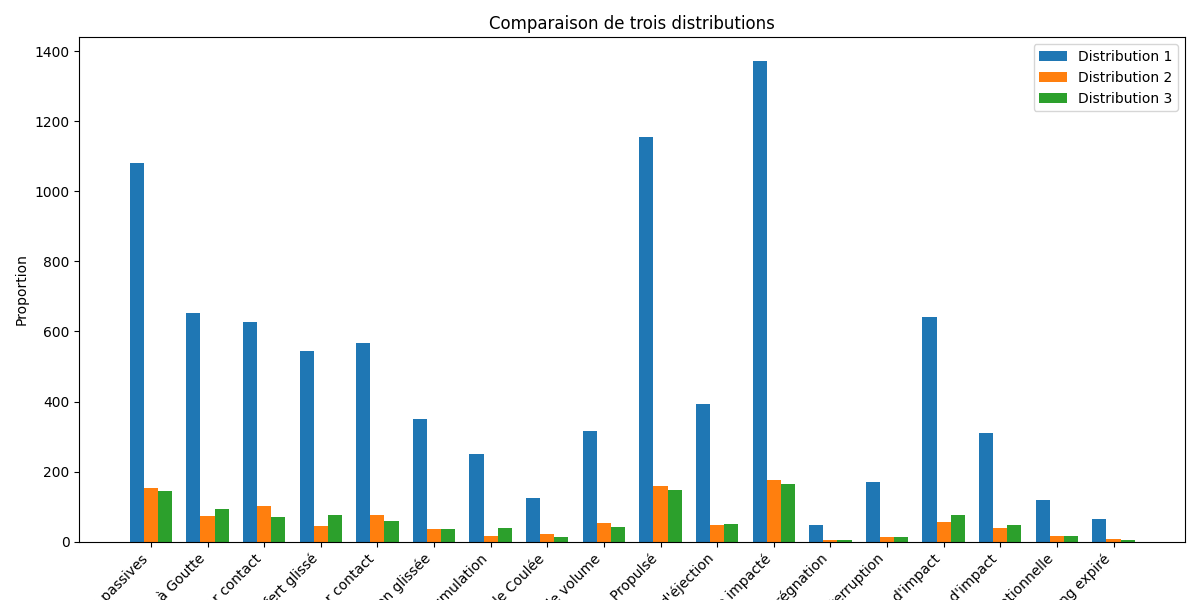
\includegraphics[width=0.7\linewidth]{../asset/distribution_train_val_test.png}
    \caption{Distribution des données de laboratoire sur les 18 classes selon le dataset d'entraînement, de validation et de test.}
    \label{fig:distribution labo}
\end{figure}

\subsection{Données réelles issues de scènes de crime}
Après l'élaboration de nos éventuels modèles pour la problématique traitée, nous avons pu manipuler des données dites réelles. Ce sont des données prises directement sur les scènes de crimes, qui sont composées de 245 images. Les images sont alors relativement moins consistantes et plus hétérogènes que les données de laboratoire. En effet, ces images sont donc issues de prises réalisées le plus souvent par la police scientifique, qui ne prend pas en compte les conditions consistantes de prise de photo respectées dans les données de laboratoire prises par Philippe Esperança. La Figure~\ref{fig: reals images} montre des exemples d'images réelles. On peut dès maintenant s'apercevoir que ces données vont être beaucoup plus compliquées à analyser pour nos modèles de deep learning au vu des nombreux objets présents sur les photos.

\begin{figure}[ht]
    \centering
    \begin{subfigure}{0.35\linewidth}
        \centering
        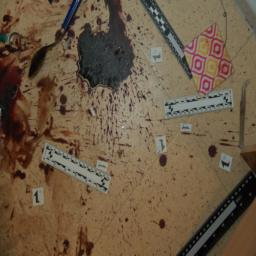
\includegraphics[width=\linewidth]{../asset/data_real/12.jpg}
        \caption{Modèle Volume Impacté}
    \end{subfigure}
    \begin{subfigure}{0.35\linewidth}
        \centering
        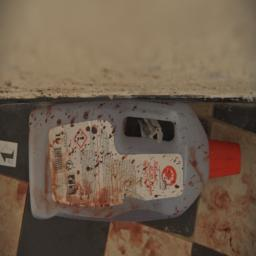
\includegraphics[width=\linewidth]{../asset/data_real/15.jpg}
        \caption{Modèle d'impact}
    \end{subfigure}
    \caption{Deux images de scènes de crime}
    \label{fig: reals images}
\end{figure}

Nous avons réparti ces données réelles à 60\% dans nos données d'entraînement, à 10\% dans nos données de validation et à 30\% dans nos données de test. En effet, une plus grande proportion d'images a été attribuée au test des données réelles afin d'avoir un test relativement plus représentatif. Cet ensemble de données de test est composé de 73 images. La Figure~\ref{fig:distribution real} nous montre la distribution des données réelles sur chacune des classes et chacun des datasets.

\begin{figure}[ht]
    \centering
    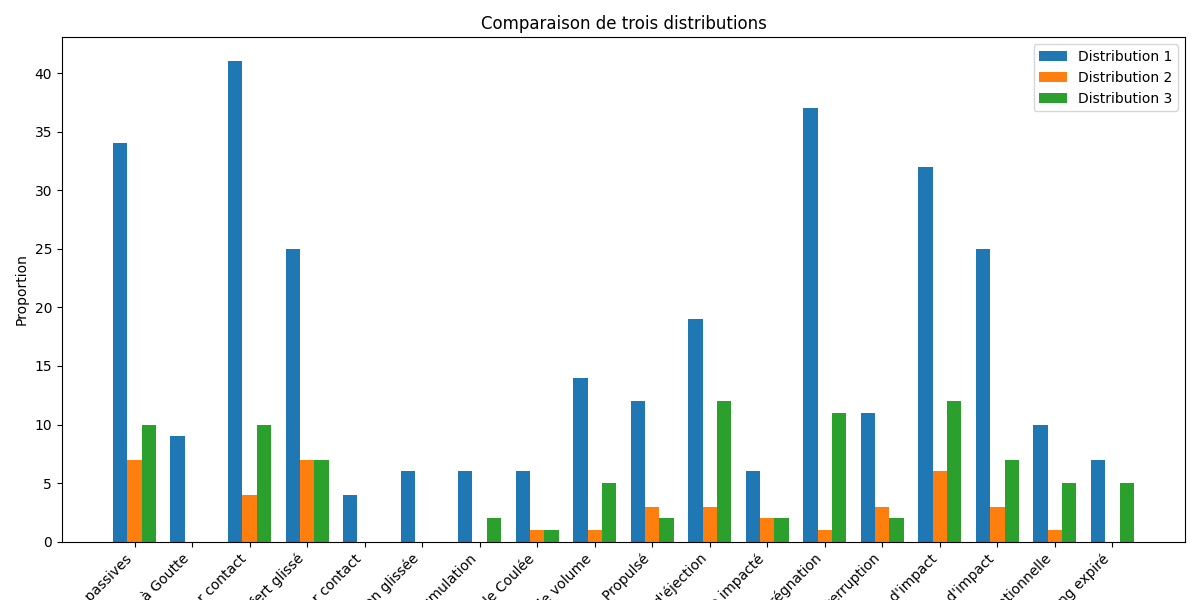
\includegraphics[width=0.7\linewidth]{../asset/distribution_train_val_test_real.png}
    \caption{Distribution des données de scène de crimes selon le dataset d'entraînement, de validation et de test.}
    \label{fig:distribution real}
\end{figure}

\subsection{Data Processing}
Les images que l'on a reçues sont en couleurs et ont une taille variable allant de $2000\times2000$ à $10000\times10000$ pixels. Nous avons donc redimensionné toutes nos images en $256\times256$. Pour l'entraînement de nos modèles deep learning, nous avons fait des symétries horizontales et verticales. Nous n'avons pas fait de rotation sur les images, car Philippe Esperança nous a expliqué qu'il ne prenait que des photos en face des taches de sang (donc sans rotation). Donc il n'est pas nécessaire d'apprendre les rotations des images. Nous avons aussi joué sur le contraste et la luminescence des images. Pour la validation, le test et l'inférence, nous n'avons pas mis de data augmentation.


\section{Modèles}
Pour aborder l'analyse de traces de sang, nous avons décidé d'utiliser le modèle Resnet 50~\cite{ResNet} pré-entraîné sur ImageNet selon certains poids indiqués dans la bibliographie~\cite{torchvision}, selon diverses approches. Nous avons utilisé la crossentropy pour notre fonction de coût, et Adam~\cite{adam} pour l'optimizer.

\subsection{ResNet linear probe}
Nous avons dans un premier temps retiré la dernière couche dense du modèle, qui était destinée à classifier sur 1000 catégories, puis effectuer du linear probing. Nous avons donc gelé tous les poids du Resnet et nous avons remplacé la dernière couche dense par 2 couches denses (qui elles sont apprenables) pour avoir une dernière couche dense à 18 neurones\footnote{la sortie correspond alors aux 18 modèles de taches de sang.}. La couche dense intermédiaire est de taille 64, et nous avons fixé un dropout à $0.1$. La Figure~\ref{fig:resnet} représente ce modèle linear probe ResNet. Les modèles utilisant le linear probing seront désignés par LP Resnet dans la suite.

\begin{figure}[ht]
    \centering
    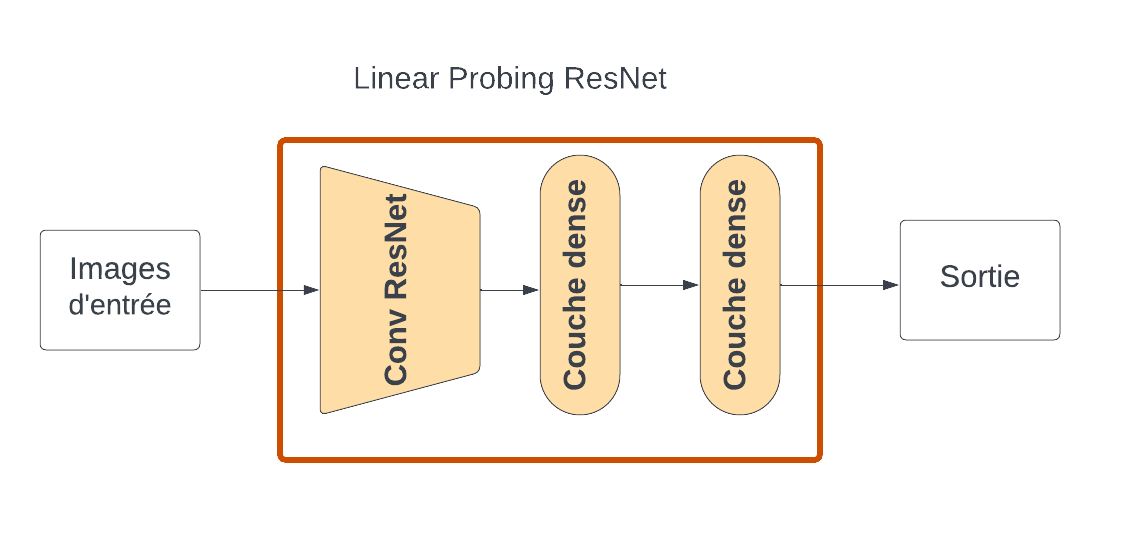
\includegraphics[width=0.7\linewidth]{../asset/Resnet.png}
    \caption{Schéma du modèle Resnet}
    \label{fig:resnet}
\end{figure}

\subsection{Réentraînement de tout le ResNet}
Nous avons également testé la méthode LP ResNet sans geler les poids de convolution du ResNet. Les modèles concernés par cette méthode seront désignés par "AWL ResNet" pour All weight learnable.

\subsection{Modèle Adversarial}

Un des points important pour la classification d'image est de pouvoir détecter la tache de sang et de la détacher du fond (background). Nous avons alors implémenté un entraînement adversarial. En plus du modèle ResNet, nous avons rajouté un modèle de MLP (Multilayer Perceptron) composé de deux couches fully connected layer qui prend en entrée la sortie de l'avant-dernière couche dense de notre Linear Probe ResNet, et prédit le background. Le but est d'alors de faire en sorte que le modèle ResNet ne possède pas d'informations sur le background de l'image dans son espace latent. La Figure~\ref{fig:resnet_adv} montre ces deux modèles. Nous appellerons cette approche "modèle Adversarial".

\begin{figure}[ht]
    \centering
    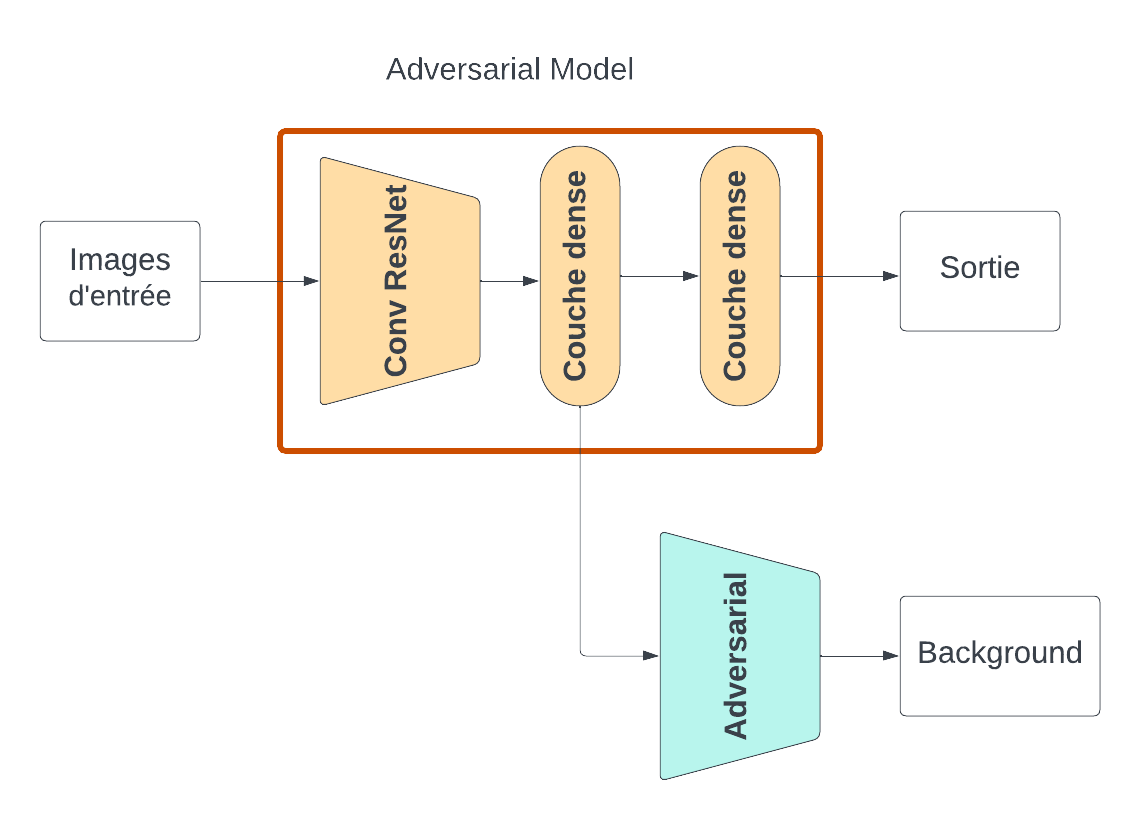
\includegraphics[width=0.7\linewidth]{../asset/Resnet_adv.png}
    \caption{Schéma du modèle Resnet adversarial}
    \label{fig:resnet_adv}
\end{figure}

Nous avons fait un entraînement adversarial pour entraîner les deux modèles simultanément. Nous avons utilisé la fonction de coût définie dans la Formule~\ref{eq: advloss}, où $CE_{tache}$ est la crossentropy entre la prédiction du modèle ResNet et la classe de la tache de sang, et $CE_{background}$ est la crossentropy de la prédiction du modèle adversarial et le background de l'image. Le paramètre $\alpha$ est un hyperparamètre que l'on va optimiser dans la section~\ref{sec: random search}.
\begin{equation}
    L_{adv} = \frac{CE_{tache}}{\alpha CE_{background}}
    \label{eq: advloss}
\end{equation}

La loss $L_{adv}$ est rétro-propagée dans le modèle ResNet tandis que la loss $CE_{background}$ est alors propagée dans le modèle adversarial.

\subsection{Fine-tune des modèles sur les données réelles}
Une fois que nous avons appris nos modèles LP ResNet et AWL ResNet sur les données de laboratoires, nous avons fine-tune ces modèles sur les données réelles (données issues de scène de crime). Nous avons appelé ces modèles respectivement FT LP Resnet et FT AWL ResNet.

Nous n'avons pas pu fine-tune le modèle Adversarial, car les taches de sang ne sont pas sur les fonds unis, et par conséquent, il n'est pas possible de fine-tune le modèle prédicteur de background sur ces données.


\section{Métriques}
Pour comparer les performances de nos modèles, nous avons utilisé les métriques suivantes : l'accuracy micro (indique le pourcentage de réussite d'un modèle), l'accuracy macro (indique la moyenne du pourcentage de réussite de chacune des classes), la précision, le rappel, le f1-score, le top~3 (indique le pourcentage de trouver la réponse parmi les 3 classes les plus prédites par le modèle). Toutes ces métriques sont des valeurs qui vont de 0 à 100, où 100 est le meilleur score. 
Les procédures de calcul de ces métriques sont explicitées en détail dans l'annexe~\ref{sec: metrics}.

\section{Apprentissage des modèles}

\subsection{Trouver le meilleur learning rate}
Afin de maximiser nos potentielles performances, nous avons commencé à effectuer un Grid-Search pour trouver le meilleur learning rate possible. Nous avons lancé l'entraînement du LP ResNet sur 5 epochs avec les learning rates suivants : $0.01, 0.005, 0.001, 0.0005, 0.0001$. La Table~\ref{tab:gridsearch} montre alors les résultats de ce Grid-Search. Pour la suite, nous avons pris un learning rate à $0.0005$.

\begin{table}[ht]
    \centering
    \begin{tabular}{cccccc}
    \toprule
    learning rate & acc micro & acc macro & f1-score & top 3 \\
    \midrule
    0.01 & 85.1 & 78.8 & 78.1 & 49.4 \\
    0.005 & 89.1 & 84.7 & 83.6 & \textbf{52.5} \\
    0.001 & 90.4 & 85.7 & 84.8 & 50.5 \\
    0.0005 & \textbf{91.1} & \textbf{86.8} & \textbf{86.0} & 49.1 \\
    0.0001 & 84.9 & 78.6 & 77.4 & 50.4 \\
    \bottomrule
    \end{tabular}
    \caption{Résultat de validation à la fin des entraînements des modèles LP ResNet avec différents learning rate.}
    \label{tab:gridsearch}
\end{table}

\subsection{Entraînement du modèle LP ResNet}
Nous avons entraîné le modèle LP ResNet sur les données de laboratoire sur 10 epochs et un learning rate de $0.0005$. La Figure~\ref{fig: train LP ResNet} montre les courbes d'apprentissage de ce modèle.

\begin{figure}[ht]
    \centering
    \begin{subfigure}{0.32\textwidth}
        \centering
        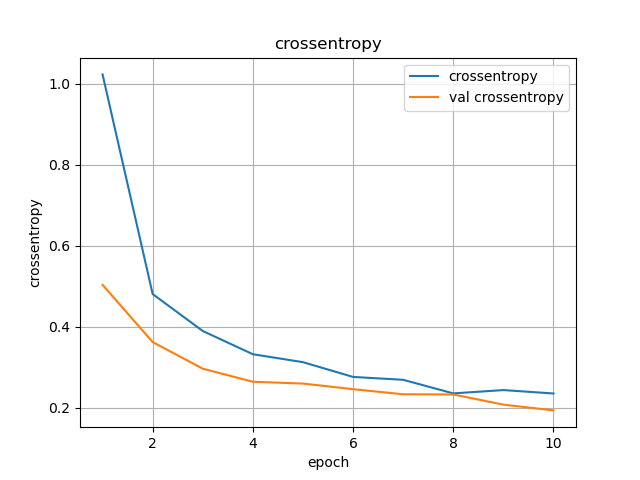
\includegraphics[width=\linewidth]{../logs/resnet_img256_0/crossentropy.png}
        \caption{crossentropy}
    \end{subfigure}
    \begin{subfigure}{0.32\textwidth}
        \centering
        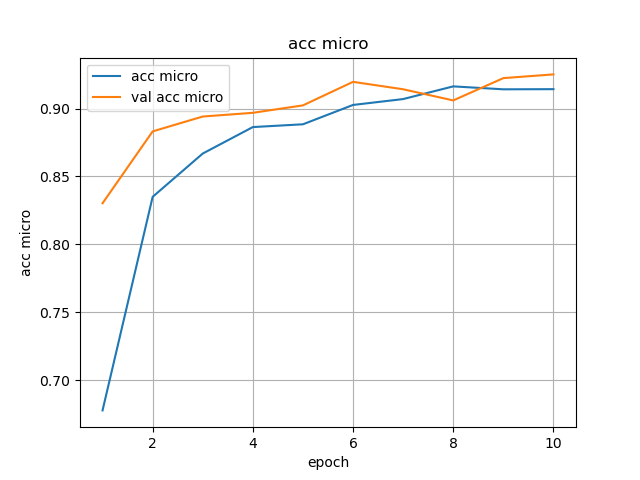
\includegraphics[width=\linewidth]{../logs/resnet_img256_0/acc micro.png}
        \caption{acc micro}
    \end{subfigure}
    \begin{subfigure}{0.32\textwidth}
        \centering
        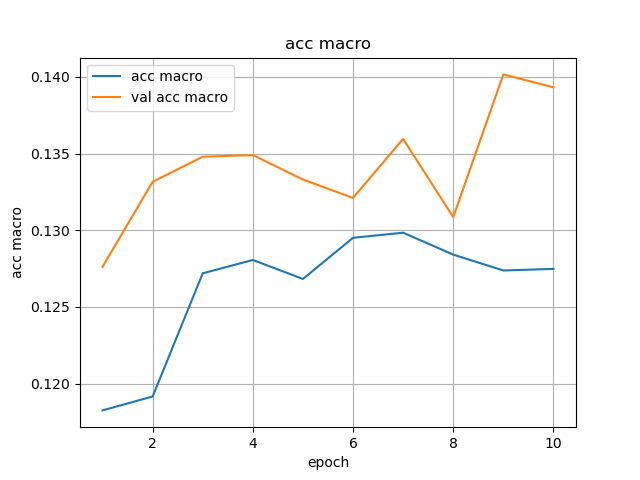
\includegraphics[width=\linewidth]{../logs/resnet_img256_0/acc macro.png}
        \caption{acc macro}
    \end{subfigure}
    \caption{Valeurs de la loss et des accuracy d'entraînement (en bleue) et de validation (en orange) en fonction des epochs durant l'entraînement du modèle LP ResNet.}
    \label{fig: train LP ResNet}
\end{figure}

\subsection{Entraînement du modèle AWL ResNet}
Nous avons entraîné le modèle LP ResNet sur les données de laboratoire sur 20 epochs. Ici, nous avons mis un learning rate de $0.0001$ pour qu'il apprenne moins vite et ne change pas trop ses paramètres dans les couches de convolutions. Nous n'avons pas pu faire une méthode de Grid Search comme le modèle de LP ResNet, en raison du temps d'apprentissage qui est plus long. La Figure~\ref{fig: train AWL ResNet} montre les courbes d'apprentissage de ce modèle.

\begin{figure}[ht]
    \centering
    \begin{subfigure}{0.32\textwidth}
        \centering
        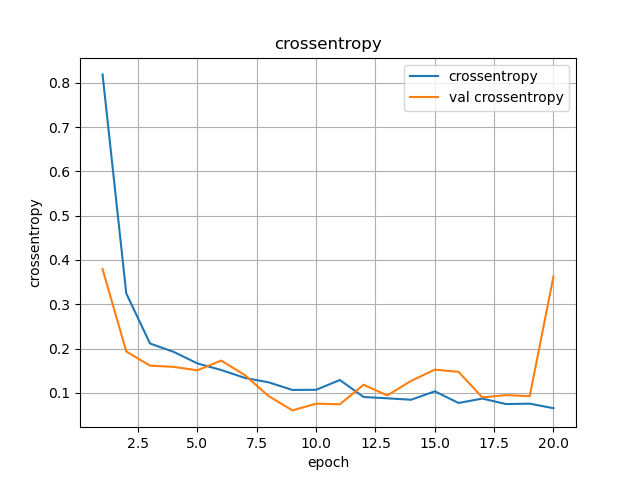
\includegraphics[width=\linewidth]{../logs/resnet_allw_img256_2/crossentropy.png}
        \caption{Crossentropy}
    \end{subfigure}
    \begin{subfigure}{0.32\textwidth}
        \centering
        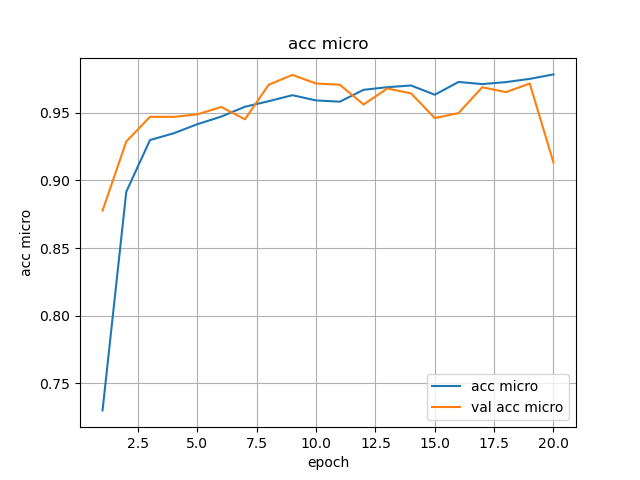
\includegraphics[width=\linewidth]{../logs/resnet_allw_img256_2/acc micro.png}
        \caption{acc micro}
    \end{subfigure}
    \begin{subfigure}{0.32\textwidth}
        \centering
        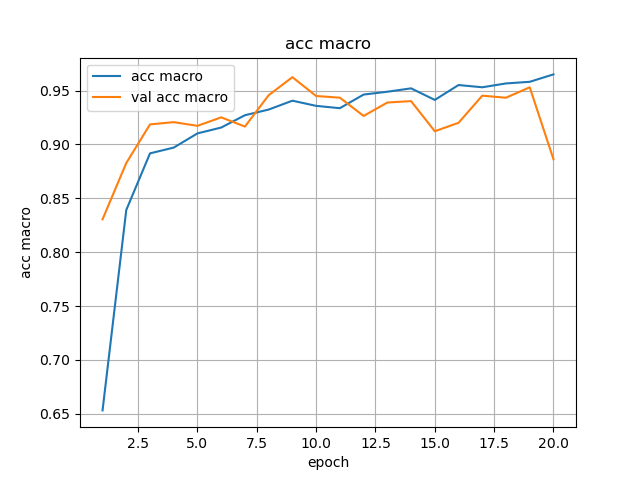
\includegraphics[width=\linewidth]{../logs/resnet_allw_img256_2/acc macro.png}
        \caption{acc macro}
    \end{subfigure}
    \caption{Valeurs de la loss et des accuracy d'entraînement (en bleue) et de validation (en orange) en fonction des epochs durant l'entraînement du modèle AWL ResNet.}
    \label{fig: train AWL ResNet}
\end{figure}

\subsection{Trouver les hyperparamètres pour le modèle Adversarial}
\label{sec: random search}
On cherche ici à trouver le meilleur learning rate pour optimiser le ResNet $lr_{res}$ et pour celui adversarial $lr_{adv}$. On cherche aussi le meilleur paramètre $\alpha$, utilisé dans la formule~\ref{eq: advloss}. On a alors implémenté un Random Search~\cite{randomsearch} et fait 10 expériences de 5 epochs, en prenant à chaque fois des paramètres dans la Table~\ref{tab:random search possibilities}\footnote{On a fait un Random Search et pas un Grid-Search, car il n'est pas possible de tester toutes les combinaisons possibles, qui sont au nombre de 200.}

\begin{table}[ht]
    \centering
    \begin{tabular}{cc}
        \toprule
        Paramètres & Valeurs possibles\\
        \midrule
        $lr_{res}$ & 0.01, 0.005, 0.001, 0.005, 0.0001\\
        $lr_{adv}$ & 0.01, 0.005, 0.001, 0.005, 0.0001\\
        $\alpha$ & 0.001, 0.1, 0.5, 1, 2, 5, 10, 100\\
        \bottomrule
    \end{tabular}
    \caption{Liste des valeurs possibles pour les hyperparamètres testés dans le Random Search}
    \label{tab:random search possibilities}
\end{table}

La Table~\ref{tab:random search results} montre les résultats de ce Random Search. \textit{res acc micro} représente l'accuracy micro de la partie ResNet (de même pour \textit{res acc macro}), et \textit{adv acc micro} représente l'accuracy micro de la partie Adversarial. Nous avons donc choisi de prendre les hyperparamètres de l'expérience numéro 2.

\begin{table}[ht]
    \centering
    \begin{tabular}{ccccccc}
    \toprule
    numéro & res acc micro & res acc macro & adv acc micro & $lr_{res}$ & $lr_{adv}$ & $\alpha$ \\
    \midrule
    0 & 79.3 & 72.8 & 82.5 & 0.1 & 1 & 10 \\
    1 & 89.6 & 84.7 & 16.1 & 0.1 & 1 & 0.1 \\
    2 & \textbf{90.8} & \textbf{86.2} & 20.2 & 0.5 & 0.01 & 0.1 \\
    3 & 85.3 & 81.2 & 44.6 & 0.1 & 1 & 0.5 \\
    4 & 88 & 85.7 & 72 & 0.5 & 0.5 & 2 \\
    5 & 89.4 & 85.4 & 56.8 & 0.01 & 0.1 & 0.5 \\
    6 & 89.5 & 85.4 & 71 & 0.1 & 0.1 & 1 \\
    7 & 87.2 & 82.2 & 71.7 & 1 & 0.01 & 1 \\
    8 & 85.3 & 80.3 & \textbf{85.3} & 0.1 & 0.5 & 10 \\
    9 & 86.7 & 83.2 & 84.8 & 0.1 & 0.01 & 10 \\
    \bottomrule
    \end{tabular}
    \caption{Résultat de validation à la fin des entraînements des modèles Adversarial avec différents hypermaramètres.}
    \label{tab:random search results}
\end{table}

\subsection{Entraînement du modèle Adversarial}
Nous avons donc entraîné le modèle Adversarial sur les données de laboratoire sur 20 epochs avec les hyperparamètres trouvés dans la section~\ref{sec: random search}. La Figure~\ref{fig: train adv} montre les courbes d'apprentissages de ce modèle.

\begin{figure}[ht]
    \centering
    \begin{subfigure}{0.32\textwidth}
        \centering
        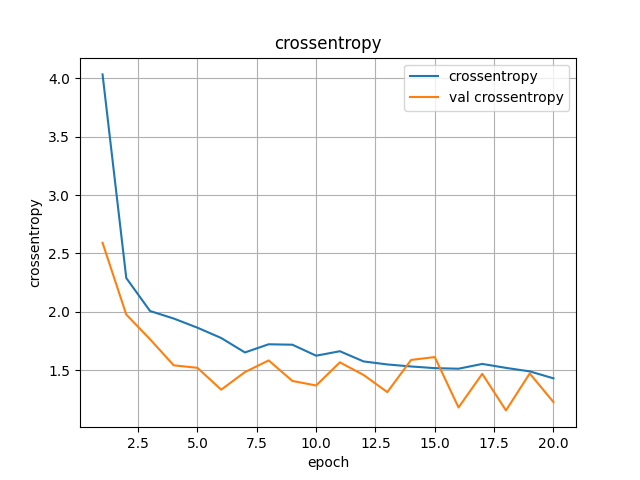
\includegraphics[width=\linewidth]{../logs/adv_img256_1/crossentropy.png}
        \caption{Loss $L_{adv}$}
    \end{subfigure}
    \begin{subfigure}{0.32\textwidth}
        \centering
        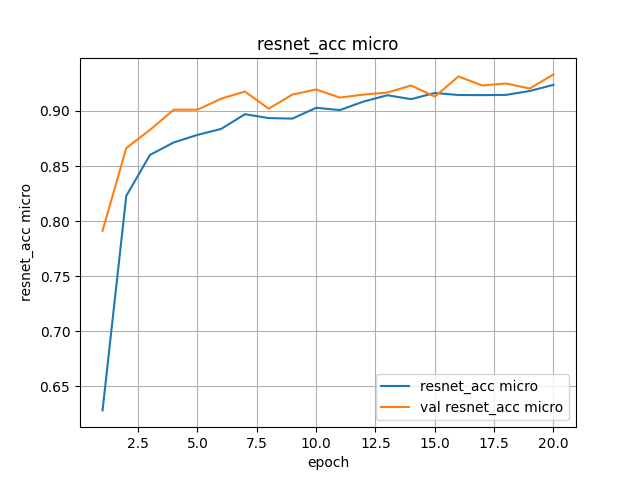
\includegraphics[width=\linewidth]{../logs/adv_img256_1/resnet_acc micro.png}
        \caption{res acc micro}
    \end{subfigure}
    \begin{subfigure}{0.32\textwidth}
        \centering
        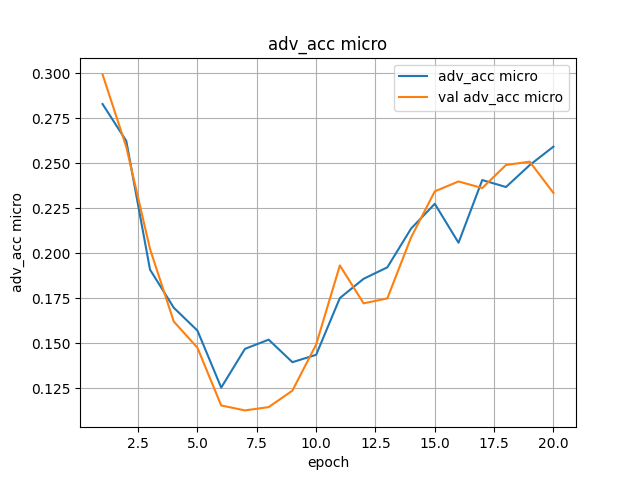
\includegraphics[width=\linewidth]{../logs/adv_img256_1/adv_acc micro.png}
        \caption{adv acc micro}
    \end{subfigure}
    \caption{Valeurs de la loss et des accuracy d'entraînement (en bleue) et de validation (en orange) en fonction des epochs durant l'entraînement du modèle Adversarial.}
    \label{fig: train adv}
\end{figure}

\subsection{Fine-tune des modèles LB ResNet et AWL ResNet}
Nous avons ensuite appris les modèles FT LB ResNet et FT AWL ResNet sur 10 epochs qui sont des modèles fine-tune sur les données réelles à partir des modèles respectivement LB ResNet et AWL ResNet sur 10 epochs. La Figure~\ref{fig: finetune} montre les courbes d'apprentissages de ce modèle.

\begin{figure}[H]
    \centering
    \begin{subfigure}{0.35\textwidth}
        \centering
        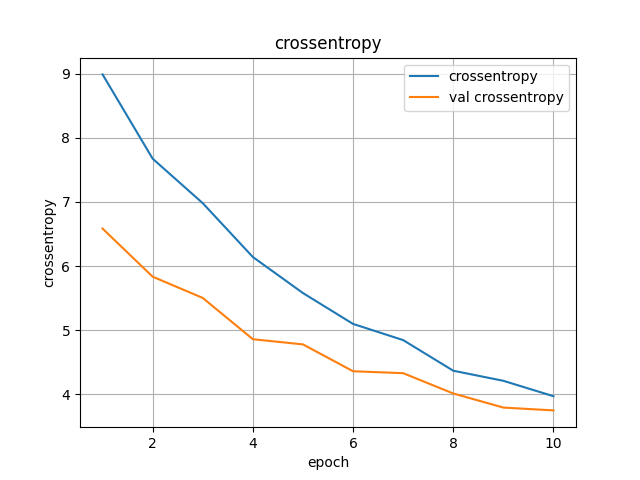
\includegraphics[width=\linewidth]{../logs/retrain_resnet_img256_0/crossentropy.png}
        \caption{crossentropy de FT LP ResNet}
    \end{subfigure}
    \begin{subfigure}{0.35\textwidth}
        \centering
        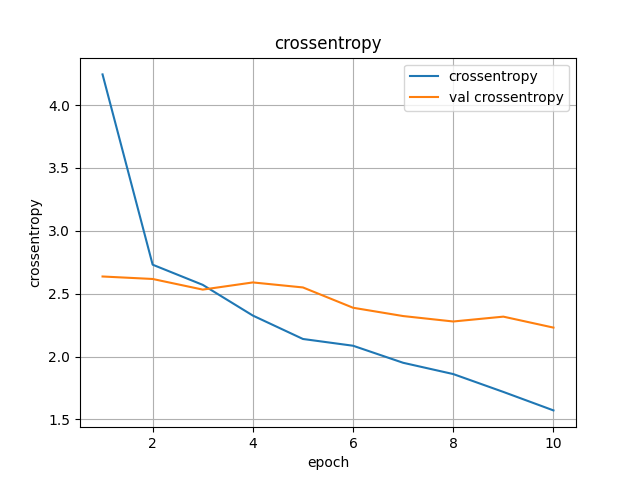
\includegraphics[width=\linewidth]{../logs/retrain_resnet_allw_img256_2/crossentropy.png}
        \caption{crossentropy de FT AWL ResNet}
    \end{subfigure}
    \caption{Valeurs de la loss d'entraînement (en bleue) et de validation (en orange) en fonction des epochs durant l'entraînement des modèles fine-tune sur les données réelles.}
    \label{fig: finetune}
\end{figure}

% \section{Interprétabilité avec les cartes de saillance}
% Afin de répondre à l'aspect "boîte noire" des réseaux de neurones, nous avons implémenté une interprétabilité dans notre modèle à l'aide de Grad-CAM~\cite{GRADCAM}. Cette méthode permet de fournir une explication visuelle vis-à-vis des décisions de classification issue de notre modèle, permettant ainsi de rajouter une certaine légitimité relative face à nos analyses de traces de sang faisant partie d'un processus judiciaire. 

\subsection{Visualisation avec Grad-CAM}
L'algorithme Grad-CAM (Gradient-weighted Class Activation Mapping) est une technique utilisée pour rendre les réseaux de neurones convolutifs (CNN) plus interprétables dans le domaine de la classification.
Il fonctionne en générant des cartes de chaleur (heatmaps) qui mettent en évidence les zones importantes d'une image qui contribuent le plus à la prédiction d'une classe spécifique.
Pour ce faire, Grad-CAM calcule les dérivées des scores de sortie de la classe cible par rapport aux caractéristiques de la dernière couche convolutive du CNN.
Ces dérivées sont ensuite globalement moyennées pour obtenir les poids d'importance de chaque carte de caractéristiques.
Enfin, les cartes de caractéristiques sont pondérées par les poids d'importance et combinées pour obtenir la carte de chaleur Grad-CAM, qui peut être superposée à l'image d'origine pour une visualisation plus intuitive.
Cette approche permet de mieux comprendre les décisions prises par le CNN et d'améliorer la confiance dans les prédictions du modèle.
La Figure~\ref{fig:grad_cam_example} montre un exemple d'une image de trace de sang avec sa carte de chaleur Grad-CAM superposée.

\begin{figure}[ht]
    \centering
    \begin{subfigure}{0.40\linewidth}
        \centering
        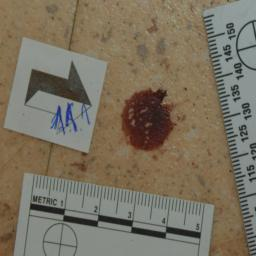
\includegraphics[width=\linewidth]{../asset/exemple/14.jpg}
    \end{subfigure}
    \begin{subfigure}{0.40\linewidth}
        \centering
        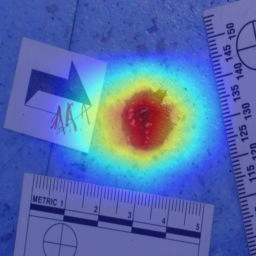
\includegraphics[width=\linewidth]{../asset/exemple/14_saliency.png}
    \end{subfigure}
    \caption{Exemple d'une image  de trace de sang (à gauche) avec sa carte de chaleur Grad CAM superposée (à droite).}
    \label{fig:grad_cam_example}
\end{figure}

En utilisant Grad-CAM, nous avons pu identifier que le modèle se focalisait parfois sur ces réglettes pour prendre sa décision, ce qui nous a permis de mieux comprendre les erreurs de classification, comme le montre la Figure~\ref{fig:grad_cam reglette}.

\begin{figure}[ht]
    \centering
    \begin{subfigure}{0.40\linewidth}
        \centering
        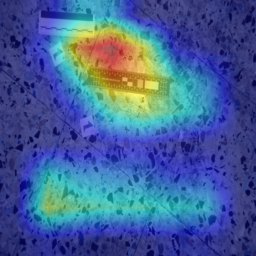
\includegraphics[width=\linewidth]{../asset/exemple/attention_reglette.jpg}
    \end{subfigure}
    \begin{subfigure}{0.40\linewidth}
        \centering
        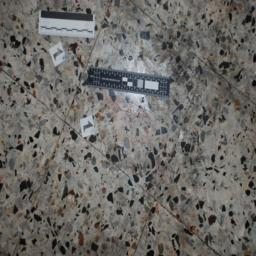
\includegraphics[width=\linewidth]{../asset/exemple/attention_reglette_image.jpg}
    \end{subfigure}
    \caption{Exemple d'une image de trace de sang (à droite) avec sa carte de chaleur Grad CAM superposée (à gauche), dans le cadre d'une attention portée à la réglette.}
    \label{fig:grad_cam reglette}
\end{figure}

\subsection{Métriques de saliency maps}
De plus, nous avons également implémenté les métriques Average Drop, Average Increase et Average Gain~\cite{opticam}, qui consiste à multiplier l'image de départ par la carte de saillence obtenue avec Grad-CAM puis de redonner cette image au modèle
pour obtenir une nouvelle prédiction. On va alors compérer le changement de probabilité de la classe prédite avant et après le masquage de l'image. Ces métriques prémettent de quantifier l'excactitude des cartes de saillance obtenues. La section~\ref{sec: grad metrics} présente les formules prémétant de les calculer.

L'Average Drop (AD) quantifie la perte de pouvoir prédictif, mesurée en termes de probabilité de classe, lorsque nous masquons uniquement l'image image. Elle est comprise entre 0 et 100, et une valeur plus faible est meilleure.

L'Average increase (AI) également connu sous le nom d'increase in confidence, mesure le pourcentage d'images pour lesquelles l'image masquée donne une probabilité de classe plus élevée que l'image originale. Elle est compris en 0 et 100, et une valeur plus haute est la meilleur.

L'Average Gain (AG) quantifie le pouvoir prédictif, mesuré en tant que probabilité de classe, lorsque nous masquons l'image. Elle est comprise entre 0 et 100, et une valeur plus élevée est meilleure.

La Table~\ref{tab:saliency_results} montre les scores de ses métriques sur la base de données de test des données réelles.

\begin{table}[ht]
    \centering
    \begin{tabular}{cccc}
        \toprule
        Métriques & Average Drop & Average Increase & Average Gain \\
        \midrule
        AWL ResNet & 91.6 & 0.0& 0.0\\
        FT AWL ResNet & 87.6 & 0.0 & 0.0\\
        \bottomrule
        \end{tabular}
    \caption{Résultats des métriques sur les données réelles (de la base de données de test).}
    \label{tab:saliency_results}
\end{table}

On peut voir dans la Table~\ref{tab:saliency_results} des résultats très peu satisefant. En effet, les deux modèles ont une Average Increase et une Average Gain de 0, ce qui signifie que avec les notations de la section~\ref{sec: grad metrics}, on a toujours $\forall i \in [1, N], p_i < o_i$. Cela signifie qu'en multipliant l'image d'origine par la carte de saillance, on obtient toujours une probabilité de classe plus faible que l'image d'origine. Cela montre que ces cartes de saillance ne sont pas fiables. Une améliorations possible serait d'utiliser des méthodes de saliency maps plus performantes comme Grad-CAM++~\cite{gradcam++} ou Score-CAM~\cite{scorecam}.


\section{Résultats}

Les résultats de test sur les données de laboratoire présent dans la Table~\ref{tab:results_lab} indiquent de meilleures performances pour le modèle Resnet qui a été réentraîné sur tous ses poids, selon l'accuracy et le F1-score. 

\begin{table}[ht]
  \centering
    \begin{tabular}{cccccc}
    \toprule
    Modèles & Acc Micro & Acc Macro & F1-score & Top 3 \\
    \midrule
    LP ResNet & 95.2 & 94.3 & 94.7 & \textbf{99.8} \\
    AWL ResNet & \textbf{97.3} & \textbf{97.1} & \textbf{96.2} & \textbf{99.8} \\
    Adversarial & 93.4 & 91.8 & 91.8 & \textbf{99.8} \\
    \bottomrule
    \end{tabular}
    \caption{Résultats de test sur les données de laboratoire}
    \label{tab:results_lab}
\end{table}

Les résultats de test sur les données de laboratoire présent dans la Table~\ref{tab: results_real} indiquent de meilleures performances pour le modèle Resnet qui était entraîné entièrement sur les données de laboratoire, puis fine-tuné sur les données réelles, selon l'accuracy et le F1-score. 
Nous avons également une valeur de Top 3 à 51.7\%, ce qui signifie qu'il y a une chance sur deux que la bonne réponse soit présente dans la prédiction. 

\begin{table}[ht]
  \centering
    \begin{tabular}{ccccccc}
    \toprule
    Modèles & Acc Micro & Acc Macro & F1-score & Top 3 \\
    \midrule
    LP ResNet & 12.9 & 6.0 & 4.0 & 19.0 \\
    FT LP ResNet & 11.8 & 6.1 & 6.4 & 26.0 \\
    AWL Resnet & 17.2 & 13.8 & 8.1 & 28.7 \\
    FT AWL ResNet & \textbf{41.9} & \textbf{33.4} & \textbf{26.9} & \textbf{51.7} \\
    Adversarial & 11.8 & 5.7 & 3.7 & 16.7 \\
    \bottomrule
    \end{tabular}
    \caption{Résultats de test sur les données réelles}
    \label{tab: results_real}
\end{table}

Le modèle Adversarial a des performances assez décevantes par rapport à un modèle Resnet, donc le modèle Adversarial n'est pas le plus adapté pour notre problématique.

Le AWL Resnet a étonnament de meilleures performances que le modèle Resnet appliquant le Linear Probing. 


\section{Interprétabilité avec les cartes de saillance}
Afin de répondre à l'aspect "boîte noire" des réseaux de neurones, nous avons implémenté une interprétabilité dans notre modèle à l'aide de Grad-CAM~\cite{GRADCAM}. Cette méthode permet de fournir une explication visuelle vis-à-vis des décisions de classification issue de notre modèle, permettant ainsi de rajouter une certaine légitimité relative face à nos analyses de traces de sang faisant partie d'un processus judiciaire. 

\subsection{Visualisation avec Grad-CAM}
L'algorithme Grad-CAM (Gradient-weighted Class Activation Mapping) est une technique utilisée pour rendre les réseaux de neurones convolutifs (CNN) plus interprétables dans le domaine de la classification.
Il fonctionne en générant des cartes de chaleur (heatmaps) qui mettent en évidence les zones importantes d'une image qui contribuent le plus à la prédiction d'une classe spécifique.
Pour ce faire, Grad-CAM calcule les dérivées des scores de sortie de la classe cible par rapport aux caractéristiques de la dernière couche convolutive du CNN.
Ces dérivées sont ensuite globalement moyennées pour obtenir les poids d'importance de chaque carte de caractéristiques.
Enfin, les cartes de caractéristiques sont pondérées par les poids d'importance et combinées pour obtenir la carte de chaleur Grad-CAM, qui peut être superposée à l'image d'origine pour une visualisation plus intuitive.
Cette approche permet de mieux comprendre les décisions prises par le CNN et d'améliorer la confiance dans les prédictions du modèle.
La Figure~\ref{fig:grad_cam_example} montre un exemple d'une image de trace de sang avec sa carte de chaleur Grad-CAM superposée.

\begin{figure}[ht]
    \centering
    \begin{subfigure}{0.40\linewidth}
        \centering
        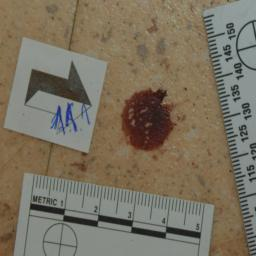
\includegraphics[width=\linewidth]{../asset/exemple/14.jpg}
    \end{subfigure}
    \begin{subfigure}{0.40\linewidth}
        \centering
        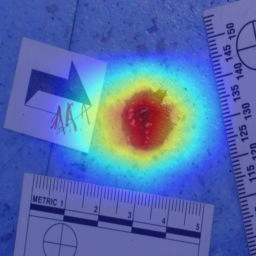
\includegraphics[width=\linewidth]{../asset/exemple/14_saliency.png}
    \end{subfigure}
    \caption{Exemple d'une image  de trace de sang (à gauche) avec sa carte de chaleur Grad CAM superposée (à droite).}
    \label{fig:grad_cam_example}
\end{figure}

En utilisant Grad-CAM, nous avons pu identifier que le modèle se focalisait parfois sur ces réglettes pour prendre sa décision, ce qui nous a permis de mieux comprendre les erreurs de classification, comme le montre la Figure~\ref{fig:grad_cam reglette}.

\begin{figure}[ht]
    \centering
    \begin{subfigure}{0.40\linewidth}
        \centering
        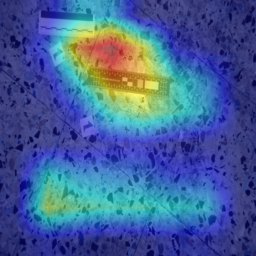
\includegraphics[width=\linewidth]{../asset/exemple/attention_reglette.jpg}
    \end{subfigure}
    \begin{subfigure}{0.40\linewidth}
        \centering
        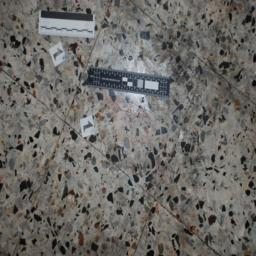
\includegraphics[width=\linewidth]{../asset/exemple/attention_reglette_image.jpg}
    \end{subfigure}
    \caption{Exemple d'une image de trace de sang (à droite) avec sa carte de chaleur Grad CAM superposée (à gauche), dans le cadre d'une attention portée à la réglette.}
    \label{fig:grad_cam reglette}
\end{figure}

\subsection{Métriques de saliency maps}
De plus, nous avons également implémenté les métriques Average Drop, Average Increase et Average Gain~\cite{opticam}, qui consiste à multiplier l'image de départ par la carte de saillence obtenue avec Grad-CAM puis de redonner cette image au modèle
pour obtenir une nouvelle prédiction. On va alors compérer le changement de probabilité de la classe prédite avant et après le masquage de l'image. Ces métriques prémettent de quantifier l'excactitude des cartes de saillance obtenues. La section~\ref{sec: grad metrics} présente les formules prémétant de les calculer.

L'Average Drop (AD) quantifie la perte de pouvoir prédictif, mesurée en termes de probabilité de classe, lorsque nous masquons uniquement l'image image. Elle est comprise entre 0 et 100, et une valeur plus faible est meilleure.

L'Average increase (AI) également connu sous le nom d'increase in confidence, mesure le pourcentage d'images pour lesquelles l'image masquée donne une probabilité de classe plus élevée que l'image originale. Elle est compris en 0 et 100, et une valeur plus haute est la meilleur.

L'Average Gain (AG) quantifie le pouvoir prédictif, mesuré en tant que probabilité de classe, lorsque nous masquons l'image. Elle est comprise entre 0 et 100, et une valeur plus élevée est meilleure.

La Table~\ref{tab:saliency_results} montre les scores de ses métriques sur la base de données de test des données réelles.

\begin{table}[ht]
    \centering
    \begin{tabular}{cccc}
        \toprule
        Métriques & Average Drop & Average Increase & Average Gain \\
        \midrule
        AWL ResNet & 91.6 & 0.0& 0.0\\
        FT AWL ResNet & 87.6 & 0.0 & 0.0\\
        \bottomrule
        \end{tabular}
    \caption{Résultats des métriques sur les données réelles (de la base de données de test).}
    \label{tab:saliency_results}
\end{table}

On peut voir dans la Table~\ref{tab:saliency_results} des résultats très peu satisefant. En effet, les deux modèles ont une Average Increase et une Average Gain de 0, ce qui signifie que avec les notations de la section~\ref{sec: grad metrics}, on a toujours $\forall i \in [1, N], p_i < o_i$. Cela signifie qu'en multipliant l'image d'origine par la carte de saillance, on obtient toujours une probabilité de classe plus faible que l'image d'origine. Cela montre que ces cartes de saillance ne sont pas fiables. Une améliorations possible serait d'utiliser des méthodes de saliency maps plus performantes comme Grad-CAM++~\cite{gradcam++} ou Score-CAM~\cite{scorecam}.


\section{Conclusion}

Le modèle sur lequel nous avons abouti représente un potentiel. Il présente de bonnes performances sur les données de laboratoires, 97\% d'accuracy (micro) contre 41\% avec les données réelles, sachant qu'il y a 10 000 images de laboratoire contre environ 300 images réelles.
D'autres pistes d'améliorations possibles concernent le modèle Resnet utilisé. Celui qui a été manipulé est le Resnet50, qui est relativement petit par rapport à d'autres Resnet plus grands existants, comme ResNet50x4, ResNet50x16. Il y a également peu de résultats concluants et significatifs à travers les cartes de saillance avec le Grad cam utilisé. Il serait éventuellement plus judicieux d'utiliser des méthodes plus sophistiqué comme Grad cam ++ ou Score cam. Une autre approche qu'on pourrait envisager est d'utiliser de l'apprentissage auto-supervisé pour exploiter l'ensemble des images non classées que possède l'expert criminalistique. En effet, depuis 10 ans, il accumule une très grande quantité d'images de scènes de crime, qui n'a pas le temps de classer, qui pourraient être utilisées pour entraîner un modèle de deep learning.

Nous avons eu l'occasion de tester d'autres approches qui sont décrites plus en détail dans la section~\ref{sec: pistes infructruces}. Parmi celles-ci, figurait l'utilisation de la clé de détermination élaborée par Philippe Esperança. Cette méthode consiste à analyser différentes caractéristiques observées sur l'image de la trace de sang, telles que la présence ou non d'une forme ovale, afin de classifier les traces de sang en différentes catégories selon les indications de la clé de détermination. Toutefois, les méthodes examinées n'ont pas donné de résultats concluants.

Notre encadrant a pu recevoir notre projet sous la forme d'une interface qui fonctionne localement sur son appareil de travail. Ce modèle d'analyse de traces de sang ne doit pas avoir accès à internet afin d'éviter tout risque d'attaque ou de fuite de données. Pouvoir faire tourner le projet en local pour l'expert criminalistique lui permet de nous faire confiance vis-à-vis de l'outil implémenté. Malgré des prédictions et des interprétations instables dans le contexte de notre projet, il a pu néanmoins apprécier et être satisfait de notre rendu dans son ensemble pour les objectifs qu'il remplit.

Notre projet va faire l'objet d'une reprise dans le cadre d'un sujet de stage au laboratoire LIS. Ainsi, notre projet possède un GitHub public ainsi qu'une documentation détaillée afin que les prochaines personnes en charge puissent reprendre aisément notre travail.

\newpage
\printbibliography

% \newpage
\begin{appendices}

\section{Images de laboratoire}
\label{sec: annexe}
\begin{table}[H]
    \centering
    \begin{tabular}{ccc}
        % \hline
        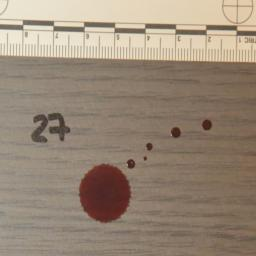
\includegraphics[width=0.20\linewidth]{../asset/data_labo/1_bois_350.jpg} & 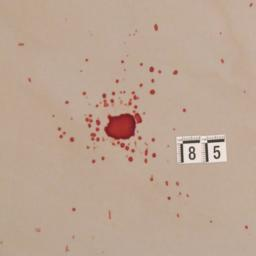
\includegraphics[width=0.20\linewidth]{../asset/data_labo/2_carrelage_523.jpg}& 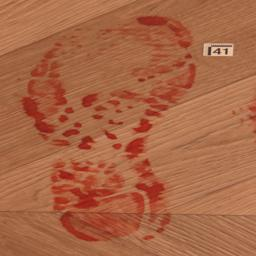
\includegraphics[width=0.20\linewidth]{../asset/data_labo/3_lino_888.jpg} \\
        1- Traces passives & 2- Goutte à Goutte & 3- Transfert par contact \\
        % \hline
        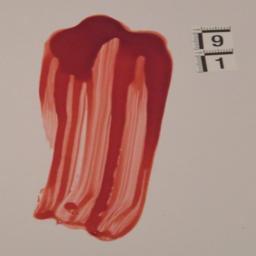
\includegraphics[width=0.20\linewidth]{../asset/data_labo/4_papier_1586.jpg} & 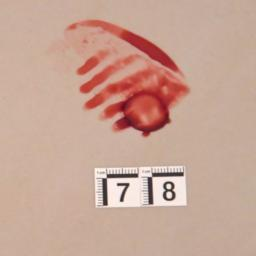
\includegraphics[width=0.20\linewidth]{../asset/data_labo/5_carrelage_5605.jpg} & 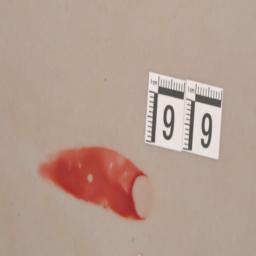
\includegraphics[width=0.20\linewidth]{../asset/data_labo/6_bois_604.jpg} \\
        4- Transfert glissé & 5- Altération par contact & 6- Altération glissée \\
        % \hline
        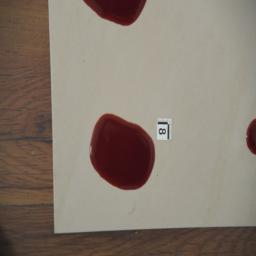
\includegraphics[width=0.20\linewidth]{../asset/data_labo/7_carrelage_5507.jpg} & \includegraphics[width=0.20\linewidth]{../asset/data_labo/8_coulée_4526.jpg} & 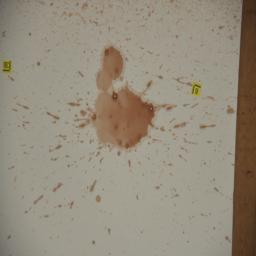
\includegraphics[width=0.20\linewidth]{../asset/data_labo/9_papier_6375.jpg} \\
        7- Accumulation & 8- Coulée & 9- Chute de volume \\
        % \hline
        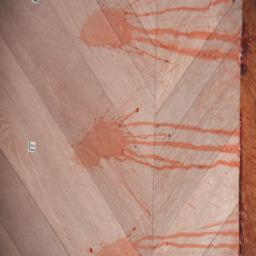
\includegraphics[width=0.20\linewidth]{../asset/data_labo/10_lino_933.jpg} & 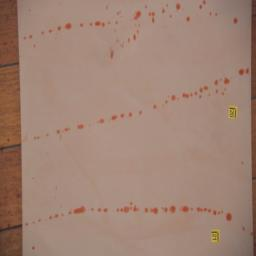
\includegraphics[width=0.20\linewidth]{../asset/data_labo/11_carrelage_905.jpg} & 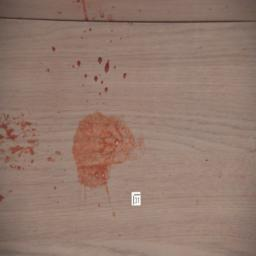
\includegraphics[width=0.20\linewidth]{../asset/data_labo/12_bois_326.jpg} \\
        10- Sang Propulsé & 11- éjection & 12- Volume impacté \\
        % \hline
        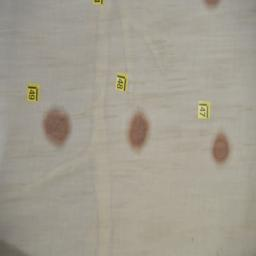
\includegraphics[width=0.20\linewidth]{../asset/data_labo/13_carrelage_7374.jpg} & 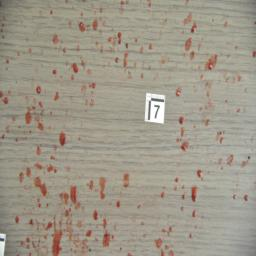
\includegraphics[width=0.20\linewidth]{../asset/data_labo/14_lino_6320.jpg} & 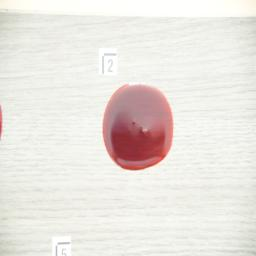
\includegraphics[width=0.20\linewidth]{../asset/data_labo/15_p1040.jpg} \\
        13- Imprégnation & 14- Zone d'interruption & 15- Modèle d'impact \\
        % \hline
        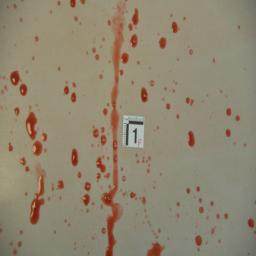
\includegraphics[width=0.20\linewidth]{../asset/data_labo/16_carrelage_598.jpg} & 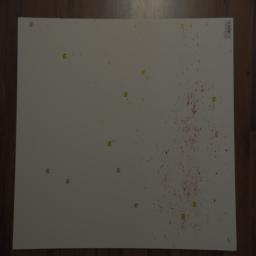
\includegraphics[width=0.20\linewidth]{../asset/data_labo/17_papier_8323.jpg} & 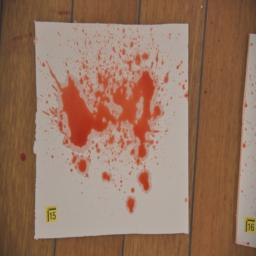
\includegraphics[width=0.20\linewidth]{../asset/data_labo/18_bois_4727.jpg}\\
        16- Foyer de modèle d'impact & 17- Trace gravitationnelle & 18- Sang expiré \\
        % \hline
    \end{tabular}
    \caption{Classe des données de laboratoire et leur exemple en image}
    \label{tab: images of all classes}
\end{table}

\section{Calcul des métriques}
\subsection{Evaluation des modèles}
\subsubsection{Accuracy micro}
L'accuracy est le pourcentage de réussite d'un modèle. Elle est calculée par la formule suivante :
\begin{equation}
    \text{Accuracy micro} = \frac{\text{Nombre de prédictions correctes}}{\text{Nombre total de prédictions}}
\end{equation}

\subsubsection{Accuracy macro}
L'accuracy macro est la moyenne des accuracy de chaque classe. Elle est calculée par la formule suivante :
\begin{equation}
    \text{Accuracy macro} = \frac{1}{N} \sum_{i=1}^{n} \frac{\text{Nombre de prédiction correctes de la classe } i}{\text{Nombre total de prédictions de la classe } i}{}
\end{equation}

\subsubsection{Précision}
La précision est le pourcentage de prédictions correctes parmi les prédictions positives. Elle est calculée par la formule suivante :
\begin{equation}
    \text{Précision} = \frac{\text{Nombre de vrais positifs}}{\text{Nombre de vrais positifs + Nombre de faux positifs}}
\end{equation}

\subsubsection{Rappel}
Le rappel est le pourcentage de prédictions correctes parmi les vrais labels positifs. Il est calculé par la formule suivante :
\begin{equation}
    \text{Rappel} = \frac{\text{Nombre de vrais positifs}}{\text{Nombre de vrais positifs + Nombre de faux négatifs}} 
\end{equation}

\subsubsection{F1-score}
Le F1-score est la moyenne harmonique de la précision et du rappel. Il est calculé par la formule suivante :
\begin{equation}
    \text{F1-score} = 2 \times \frac{\text{Précision} \times \text{Rappel}}{\text{Précision} + \text{Rappel}}
\end{equation}

\subsubsection{Top 3}
Le Top 3 est le pourcentage de trouver la réponse parmi les 3 classes les plus prédites par le modèle. Il est calculé par la formule suivante :
\begin{equation}
    \text{Top 3} = \frac{\text{Nombre de prédictions correctes parmi les 3 premières prédictions}}{\text{Nombre total d'exemples}}
\end{equation}

\subsection{Evaluation des cartes de saillance}
\label{sec: grad metrics}

Soit $p_i = \text{arg}\max_c p_i^c$ la probabilité de la classe prédicte par le modèle pour l'image $x_i$. Soit $o_i$ la probabilité de cette même classe prédite par le modèle pour l'image maské de ca carte de saillance $x_i * s_i$ (où $s_i$ est la carte de saillance de l'image $x_i$). On définie $N$ le nombre totale d'image dans le test set. On note $[x]_+$ le maximun entre $0$ et la valeur $x$ ($[x]_+=\max(0, x)$). On définie les métriques suivantes :

\subsubsection{Averare Drop (AD)}
\begin{equation}
    \text{AD} = \frac{1}{N} \sum_{i=1}^{N} \frac{[p_i - o_i]_+}{p_i} \cdot 100
\end{equation}

\subsubsection{Average Increase (AI)}
\begin{equation}
    \text{AI} = \frac{1}{N} \sum_{i=1}^{N} 1_{p_i<o_i} \cdot 100
\end{equation}

\subsubsection{Average Gain (AG)}
\begin{equation}
    \text{AG} = \frac{1}{N} \sum_{i=1}^{N} \frac{[o_i - p_i]_+}{1 - p_i} \cdot 100
\end{equation}

\section{Pistes infructueuses}
\label{sec: pistes infructruces}


\section{Pistes infructueuses}

Au cours de ce projet nous avons exploré plusieurs pistes qui se sont avérées infructueuses. Nous les présentons ici pour que le lecteur puisse comprendre les raisons pour lesquelles nous avons choisi de ne pas les poursuivre.

\subsection{Interprétabilité des modèles par feature ingenering}

Un des objectifs de ce projet était de parvenir à interpréter les choix des modèles de machine learning que nous avons entrainé.
Pour cela, nous avons tenté de nous inspirer du travail réalisé précedement par l'équipe d'experts criminalistiques. En effet,
leur approche s'inspire de la classification des espèces animales et végétales par les biologistes. Ils ont cherché à identifier des caractéristiques
déterminantes pour chaques traces de sang et ainsi à classifier les traces de sang grâce à un arbre de décision
portant sur ces caractéristiques (par exemple: la forme, la taille, présence de tâches milimétriques près des tâches centimétriques, etc..).
Nous avons donc tenté de reproduire cette approche en utilisant des techniques de feature ingenering pour extraire des caractéristiques
fondamentales des traces de sang souis formes de critères mathématico-géométriques. Pour cela nous avons d'abord tenté de réaliser
un algorithme de segmentation non-supervisé par détection de contours pour extraire les formes des tâches de sang, avec des résultats peu concluants. Nous avons ensuite
tenté de réaliser un algorithme melant des techniques de traitement d'images (seuils, ect..), d'apprentissage auto-supervisé (Unet) et de géométrie pour extraire des caractéristiques géométriques telle la taille
des tâche satellitaires par rapport à la tâche centrale, la forme des tâches (critère d'ovoidité, de circularité, etc..). Ces tentatives ont néanmoins
été infructueuses, car les masques de segmentation était trop imprécis du fait de la grande variabilité des images de tâches de sang. Nous avons également tenté des méthodes de segmentation
adversariale en tirant partie du fait que nous connaissions pour toute les images la nature du support (bois,lino,carrelage,etc..) pour tenter de segmenter les tâches de sang par une approche faiblement supervisée. Ces tentatives ont également été infructueuses, car nous 
avions peu de donnée d'entrainement ce qui rendait tout apprentissage trop instable de manière faiblement supervisée.

Nous avons également tenté d'extraire ces caractéristiques (masques de segmentation, critères géométriques) à l'aide de modèle de deep learning
utilisant des techniques dites de "zero-shot classification" (modèles de type CLIP-ViT, etc..) ou zero-shot segmentation (SegmentAnything). Ces tentatives ont également été infructueuses, car le manque de contraste
sur certaines images de tâches de sang ou leur trop grand éclatement rendait les masques de segmentation trop imprécis.






\end{appendices}

\end{document}